\section{Vorüberlegungen}

\subsection{Datenquellen}
Ein Kernpunkt für die Entwicklung der Ingestion-Schnittstelle ist die Analyse der möglichen Datenquellen.
Da das System alle möglichen Datenquellen unterstützen soll, werden hier mögliche Typen dargestellt, mit denen sich alle Datenquellen abdecken lassen.
Dazu werden Merkmale betrachtet die Art und der Typ Ingestion bestimmen.
Mit der Art wird hier bezeichnet, ob die verwendeten Daten strukturiert, semi- oder unstrukturiert sind.
Da in der Vorarbeit, dem Masterprojekt, \textit{Apache Spark} verwendet wurde, ist dieser Punkt bereits abgedeckt und fällt bei der Entwicklung nicht weiter ins Gewicht.

Als zweites gibt es die Typen, die hier beschreiben, wie Daten in das System gelangen.
Dazu gibt es zwei Merkmale, in denen sich die Ingestions unterscheiden können.
Das erste ist, ob die Unterscheidung zwischen Push- und Pull-Prinzip.
Bei dem Push-Prinzip werden die zu speichernden Daten mit der Anfrage an das System gesendet und bei dem Pull-Prinzip muss dass System die Daten aus einer Quelle laden.
Die zweite Unterscheidung findet statt in einmalige in kontinuierliche Ingestion.
Diese Unterscheidungen können, müssen aber nicht, von der Datenquelle abhängig sein.
Als Beispiel gibt es Datenströme, die laufend Daten senden und somit eine Ingestion benötigen, die auch laufend Daten annimmt.
Im Gegensatz dazu gibt es Datenbanken, bei denen das System die Daten aus der Quelle laden muss und somit die Ingestion sowohl einmalig als auch kontinuierlich sein kann.

Aus diesen Unterscheidungen ergeben sich die vier mögliche Verarbeitungswege, die in \ref{fig:ingestion_types} zu sehen sind.
Sowohl für Push- und Pull-Prinzip kann eine einfache Ingestion ausgeführt werden, die sich für kontinuierliche Pull-Ingestions wiederholt.
Bei einer kontinuierlichen Ingestion, bei der Daten an das System gesendet werden, handelt es sich um Datenströme, die eine extra Verarbeitung erfordern.

\begin{figure}
  \centering
  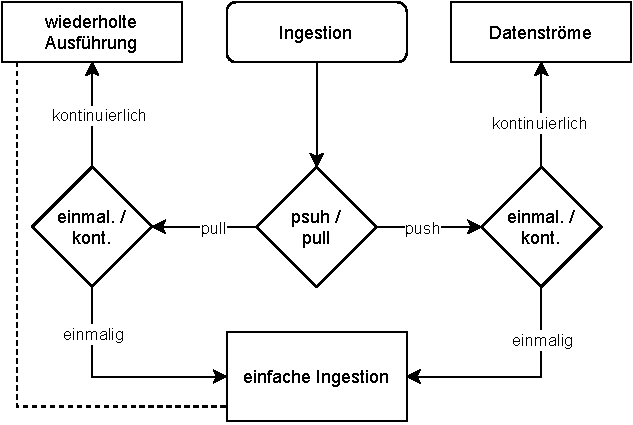
\includegraphics{Grafiken/ingestion-types.pdf}
  \caption{Ingestion-Typen}
  \label{fig:ingestion_types}
\end{figure}
